\documentclass[
11pt, % The default document font size, options: 10pt, 11pt, 12pt
%codirector, % Uncomment to add a codirector to the title page
]{charter} 




% El títulos de la memoria, se usa en la carátula y se puede usar el cualquier lugar del documento con el comando \ttitle
\titulo{ ADCS - Attitude determination control system board} 

% Nombre del posgrado, se usa en la carátula y se puede usar el cualquier lugar del documento con el comando \degreename
\posgrado{Carrera de Especialización en Sistemas Embebidos} 
%\posgrado{Carrera de Especialización en Internet de las Cosas} 
%\posgrado{Carrera de Especialización en Intelegencia Artificial}
%\posgrado{Maestría en Sistemas Embebidos} 
%\posgrado{Maestría en Internet de las cosas}

% Tu nombre, se puede usar el cualquier lugar del documento con el comando \authorname
\autor{Valdez Gastón} 

% El nombre del director y co-director, se puede usar el cualquier lugar del documento con el comando \supname y \cosupname y 
%y \pertecosupname
%\pertesupname{Aerospace Laboratory} 
\director{Amilcar Rincón Charris}
\pertenenciaDirector{Aerospace Laboratory} 
% FIXME:NO IMPLEMENTADO EL CODIRECTOR ni su pertenencia
%\codirector{John Doe} % para que aparezca en la portada se debe descomentar la opción codirector en el documentclass
%\pertenenciaCoDirector{FIUBA}

% Nombre del cliente, quien va a aprobar los resultados del proyecto, se puede usar con el comando \clientename y \empclientename
\cliente{Amilcar Rincon Charris}
\empresaCliente{Aerospace Laboratory}
%\pertesupname{lalallal}
% Nombre y pertenencia de los jurados, se pueden usar el cualquier lugar del documento con el comando \jurunoname, \jurdosname y \jurtresname y \perteunoname, \pertedosname y \pertetresname.
\juradoUno{Nombre y Apellido (1)}
\pertenenciaJurUno{pertenencia (1)} 
\juradoDos{Nombre y Apellido (2)}
\pertenenciaJurDos{pertenencia (2)}
\juradoTres{Nombre y Apellido (3)}
\pertenenciaJurTres{pertenencia (3)}
 
\fechaINICIO{30 de abril de 2021}		%Fecha de inicio de la cursada de GdP \fechaInicioName
\fechaFINALPlan{18 de junio de 2021} 	%Fecha de final de cursada de GdP
\fechaFINALTrabajo{15 de mayo de 2022}	%Fecha de defensa pública del trabajo final


\begin{document}

\maketitle
\thispagestyle{empty}
\pagebreak


\thispagestyle{empty}
{\setlength{\parskip}{0pt}
\tableofcontents{}
}
\pagebreak


\section*{Registros de cambios}
\label{sec:registro}


\begin{table}[ht]
\label{tab:registro}
\centering
\begin{tabularx}{\linewidth}{@{}|c|X|c|@{}}
\hline
\rowcolor[HTML]{C0C0C0} 
Revisión & \multicolumn{1}{c|}{\cellcolor[HTML]{C0C0C0}Detalles de los cambios realizados} & Fecha      \\ \hline
0      & Creación del documento                                 &\fechaInicioName \\ \hline
%1      & Se completa hasta el punto 4 inclusive                 & dd/mm/aaaa \\ \hline
%2      & Se completa hasta el punto 7 inclusive
%		  Se puede agregar algo más \newline
%		  En distintas líneas \newline
%		  Así                                                    & dd/mm/aaaa \\ \hline
%3      & Se completa hasta el punto 11 inclusive                & dd/mm/aaaa \\ \hline
%4      & Se completa el plan	                                 & dd/mm/aaaa \\ \hline
\end{tabularx}
\end{table}

\pagebreak



\section*{Acta de constitución del proyecto}
\label{sec:acta}

\begin{flushright}
Buenos Aires, \fechaInicioName
\end{flushright}

\vspace{2cm}

Por medio de la presente se acuerda con el Ing. \authorname\hspace{1px} que su Trabajo Final de la \degreename\hspace{1px} se titulará ``\ttitle'', consiste  en el diseño electrónico de un módulo  Attitude determination control systems para introducirse en un cubesat.  
 con fecha de inicio \fechaInicioName\hspace{1px} y fecha de presentación pública \fechaFinalName.

Se adjunta a esta acta la planificación inicial.

\vfill

% Esta parte se construye sola con la información que hayan cargado en el preámbulo del documento y no debe modificarla
\begin{table}[ht]
\centering
\begin{tabular}{ccc}
\begin{tabular}[c]{@{}c@{}}Dr. Ing. Ariel Lutenberg \\ Director posgrado FIUBA\end{tabular} & \hspace{2cm} & \begin{tabular}[c]{@{}c@{}}\clientename \\ \empclientename \end{tabular} \vspace{2.5cm} \\ 
\multicolumn{3}{c}{\begin{tabular}[c]{@{}c@{}} \supname \\ Director del Trabajo Final\end{tabular}} \vspace{2.5cm} \\
%\begin{tabular}[c]{@{}c@{}}\jurunoname \\ Jurado del Trabajo Final\end{tabular}     &  & \begin{tabular}[c]{@{}c@{}}\jurdosname\\ Jurado del Trabajo Final\end{tabular}  \vspace{2.5cm}  \\
%\multicolumn{3}{c}{\begin{tabular}[c]{@{}c@{}} \jurtresname\\ Jurado del Trabajo Final\end{tabular}} \vspace{.5cm}                                                                     
\end{tabular}
\end{table}




\section{1. Descripción técnica-conceptual del proyecto a realizar}
\label{sec:descripcion}

Un cubesat es un satélite que posee una estructura de 10x10x10 cm y que posee un peso máximo de 1,33 kg. Los satélites cubesat permiten que distintos investigadores y entusiastas del espacio envien satélites al espacio con un costo relativamente bajo respecto a otro tipo de soluciones. La construcción de un  cubesat se realiza mediante módulos electrónicos ensamblados entre sí usando el conector denominado PC104. 

Un módulo electrónico que es parte de un cubesat se denomina ADCS, este es responsable de controlar y mantener la orientación del cubesat en el espacio. Este tipo de control  permite que los instrumentos que se encuentren dentro del satélite se orienten en direcciones especificas.  Por ejemplo puede orientar su antena hacia la tierra para que la comunicación con tierra tenga mayor fluidez. 

Los sistemas ADCS tienen dos tipos de sensores: de posicionamiento o inerciales. Los primeros se relacionan con el conocimiento de la posición absoluta,es decir, requiere un conocimiento del entorno. Los sensores inerciales no requieren este tipo de conocimiento, sino que, utilizan parámetros como velocidad angular o aceleración. 

Estos sistemas no solamente deben realizar la lectura de los sensores, sino que actúan sobre el sistema para orientar el satélite en la posición deseada y mantenerla estable. Esta actuación se realiza mediante ruedas de reacción o torques magnéticos para realizar ajustes cuando el satelite se encuentra orbitando la tierra.

Para generar el movimiento con el uso de ruedas de reacción o torques magnéticos, se debe  conocer la posición y orientación en el espacio del cubesat. Una vez conocidos ambos parámetros, mediante un proceso denominado “algoritmo de fusión” produce la actuación sobre las ruedas de reacción o magnetorques para orientar al cubesat en la posición deseada.

 Los sistemas ADCS se encuentran de forma comercial y  existen empresas que proveen este tipo de soluciones para los cubesats. El presente proyecto consiste en el desarrollo de un sistema ADCS. El desarrollo propio contiene las siguientes ventajas frente a las soluciones comerciales: 
\begin{itemize}
	\item Selección de torques magnéticos, ruedas de tracción o innovar en mecanismos de orientación. 
	\item Realizar distintos algoritmos y probar la eficiencia de consumo eléctrico. 
	\item Posibilidad de generar un producto comercial 
\end{itemize}


 El diagrama en bloques propuesto para el desarrollo del proyecto consiste en el diagrama de la figura \ref{fig:adcs}. El proyecto se divide en dos etapas: fase de prototipo y versión final. Una vez finalizada la fase de prototipado se realizan las pruebas de validación del sistema.  Una vez superada la etapa de validación se procede al desarrollo en su versión final y comienza la segunda fase del proyecto. 
 Cabe destacar que como subproducto puede generarse una placa comercial, siendo esto último deseable pero no exigible por parte del cliente. 

\begin{figure}[htpb]
	\centering 
	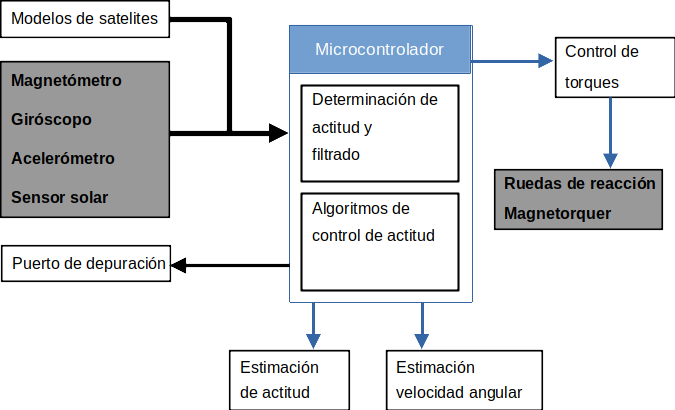
\includegraphics[width=.8\textwidth]{Figuras/sistemaadcs.png}
	\caption{Diagrama de \textit{Activity on Node}.}
	\label{fig:adcs}
\end{figure}

\section{2. Identificación y análisis de los interesados}
\label{sec:interesados}


\begin{table}[ht]
	%\caption{Identificación de los interesados}
	%\label{tab:interesados}
	\begin{tabularx}{\linewidth}{@{}|l|X|X|l|@{}}
		\hline
		\rowcolor[HTML]{C0C0C0} 
		Rol           & Nombre y Apellido & Organización 	& Puesto 	\\ \hline
		Auspiciante   &                   &              	&        	\\ \hline
		Cliente       & \clientename      &\empclientename	&        	\\ \hline
		Impulsor      &                   &              	&        	\\ \hline
		Responsable   & \authorname       & IAR        	& Alumno 	\\ \hline
		Colaboradores &                   &              	&        	\\ \hline
		Orientador    & \supname	      & \pertesupname 	& Director Trabajo final \\ \hline
		Equipo        &  -                &  -             	& -        	\\ \hline
		Opositores    &                   &              	&        	\\ \hline
		Usuario final & \supname     &      \pertesupname        	&        	\\ \hline
	\end{tabularx}
\end{table}


\section{3. Propósito del proyecto}

	El propósito del proyecto es generar el módulo electrónico del sistema ADCS para un cubesat. 

\section{4. Alcance del proyecto}
\label{sec:alcance}
\begin{itemize}
	\item Desarrollo del algoritmo ADCS 
	\item Desarrollo de software en C/C++ para el sistema embebido 
	\item Diseño y desarrollo del protocolo de comunicación utilizando el conector PC104
	\item Diseño y simulación del hardware asociado al microcontrolador 
	\item Diseño de ensayos de validación (TBD) 
	\item Generación de documentación. 
	\item Integración a un cubesat funcional(TBD)
\end{itemize}
	El alcance del proyecto no contempla la fabricación del PCB y los ensayos de validación se realizarán en un lugar a definir con el cliente. 


\section{5. Supuestos del proyecto}
\label{sec:supuestos}
\begin{itemize}
	\item Los componentes serán seleccionados y se poseen los recursos económicos para su adquisición  
	\item El sistema embebido posee disponibilidad en el mercado. 
	\item Se tienen las licencias correspondientes para los programas de simulación electrónica y diseño de PCB  
	\item Se posee acceso a pc con sistema linux/windows 
	\item El personal abocado al diseño mecánico realizará el trabajo en tiempo y forma.  
	\item Hay recursos económicos disponibles para enviar a fabricar la placa de circuito impreso. 
	\item El flujo de trabajo se define con anterioridad 
\end{itemize}

\section{6. Requerimientos}
\label{sec:requerimientos}
\begin{enumerate}
	\item Req funcional
		\begin{enumerate}
			\item posee sistema 1 
			\item posee sistem 2 
			
		\end{enumerate}

	\item Req funcional
		\begin{enumerate}
			\item posee sistema 1 
			\item posee sistem 2 	
		\end{enumerate}



\end{enumerate}



\section{7. Historias de usuarios (\textit{Product backlog})}
\label{sec:backlog}


\section{8. Entregables principales del proyecto}
\label{sec:entregables}
\begin{itemize}
	\item Archivos de simulación 
	\item Scripts de simulación 
	\item Archivos de esquemáticos en PDF y archivo original 
	\item 

\end{itemize}

\section{9. Desglose del trabajo en tareas}
\label{sec:wbs}

\section{10. Diagrama de Activity On Node}
\label{sec:AoN}



\section{11. Diagrama de Gantt}
\label{sec:gantt}

\section{12. Presupuesto detallado del proyecto}
\label{sec:presupuesto}


\begin{table}[htpb]
\centering
\begin{tabularx}{\linewidth}{@{}|X|c|r|r|@{}}
\hline
\rowcolor[HTML]{C0C0C0} 
\multicolumn{4}{|c|}{\cellcolor[HTML]{C0C0C0}COSTOS DIRECTOS} \\ \hline
\rowcolor[HTML]{C0C0C0} 
Descripción &
  \multicolumn{1}{c|}{\cellcolor[HTML]{C0C0C0}Cantidad} &
  \multicolumn{1}{c|}{\cellcolor[HTML]{C0C0C0}Valor unitario} &
  \multicolumn{1}{c|}{\cellcolor[HTML]{C0C0C0}Valor total} \\ \hline
 &
  \multicolumn{1}{c|}{} &
  \multicolumn{1}{c|}{} &
  \multicolumn{1}{c|}{} \\ \hline
 &
  \multicolumn{1}{c|}{} &
  \multicolumn{1}{c|}{} &
  \multicolumn{1}{c|}{} \\ \hline
\multicolumn{1}{|l|}{} &
   &
   &
   \\ \hline
\multicolumn{1}{|l|}{} &
   &
   &
   \\ \hline
\multicolumn{3}{|c|}{SUBTOTAL} &
  \multicolumn{1}{c|}{} \\ \hline
\rowcolor[HTML]{C0C0C0} 
\multicolumn{4}{|c|}{\cellcolor[HTML]{C0C0C0}COSTOS INDIRECTOS} \\ \hline
\rowcolor[HTML]{C0C0C0} 
Descripción &
  \multicolumn{1}{c|}{\cellcolor[HTML]{C0C0C0}Cantidad} &
  \multicolumn{1}{c|}{\cellcolor[HTML]{C0C0C0}Valor unitario} &
  \multicolumn{1}{c|}{\cellcolor[HTML]{C0C0C0}Valor total} \\ \hline
\multicolumn{1}{|l|}{} &
   &
   &
   \\ \hline
\multicolumn{1}{|l|}{} &
   &
   &
   \\ \hline
\multicolumn{1}{|l|}{} &
   &
   &
   \\ \hline
\multicolumn{3}{|c|}{SUBTOTAL} &
  \multicolumn{1}{c|}{} \\ \hline
\rowcolor[HTML]{C0C0C0}
\multicolumn{3}{|c|}{TOTAL} &
   \\ \hline
\end{tabularx}%
\end{table}


\section{13. Gestión de riesgos}
\label{sec:riesgos}

\begin{consigna}{red}
a) Identificación de los riesgos (al menos cinco) y estimación de sus consecuencias:
 
Riesgo 1: detallar el riesgo (riesgo es algo que si ocurre altera los planes previstos de forma negativa)
\begin{itemize}
	\item Severidad (S): mientras más severo, más alto es el número (usar números del 1 al 10).\\
	Justificar el motivo por el cual se asigna determinado número de severidad (S).
	\item Probabilidad de ocurrencia (O): mientras más probable, más alto es el número (usar del 1 al 10).\\
	Justificar el motivo por el cual se asigna determinado número de (O). 
\end{itemize}   

Riesgo 2:
\begin{itemize}
	\item Severidad (S): 
	\item Ocurrencia (O):
\end{itemize}

Riesgo 3:
\begin{itemize}
	\item Severidad (S): 
	\item Ocurrencia (O):
\end{itemize}


b) Tabla de gestión de riesgos:      (El RPN se calcula como RPN=SxO)

\begin{table}[htpb]
\centering
\begin{tabularx}{\linewidth}{@{}|X|c|c|c|c|c|c|@{}}
\hline
\rowcolor[HTML]{C0C0C0} 
Riesgo & S & O & RPN & S* & O* & RPN* \\ \hline
       &   &   &     &    &    &      \\ \hline
       &   &   &     &    &    &      \\ \hline
       &   &   &     &    &    &      \\ \hline
       &   &   &     &    &    &      \\ \hline
       &   &   &     &    &    &      \\ \hline
\end{tabularx}%
\end{table}

Criterio adoptado: 
Se tomarán medidas de mitigación en los riesgos cuyos números de RPN sean mayores a...

Nota: los valores marcados con (*) en la tabla corresponden luego de haber aplicado la mitigación.

c) Plan de mitigación de los riesgos que originalmente excedían el RPN máximo establecido:
 
Riesgo 1: plan de mitigación (si por el RPN fuera necesario elaborar un plan de mitigación).
  Nueva asignación de S y O, con su respectiva justificación:
  - Severidad (S): mientras más severo, más alto es el número (usar números del 1 al 10).
          Justificar el motivo por el cual se asigna determinado número de severidad (S).
  - Probabilidad de ocurrencia (O): mientras más probable, más alto es el número (usar del 1 al 10).
          Justificar el motivo por el cual se asigna determinado número de (O).

Riesgo 2: plan de mitigación (si por el RPN fuera necesario elaborar un plan de mitigación).
 
Riesgo 3: plan de mitigación (si por el RPN fuera necesario elaborar un plan de mitigación).

\end{consigna}


\section{14. Gestión de la calidad}
\label{sec:calidad}

\begin{consigna}{red}
Elija al menos diez requerientos que a su criterio sean los más importantes/críticos/que aportan más valor y para cada uno de ellos indique las acciones de verificación y validación que permitan asegurar su cumplimiento.

\begin{itemize} 
\item Req \#1: copiar acá el requerimiento.

\begin{itemize}
	\item Verificación para confirmar si se cumplió con lo requerido antes de mostrar el sistema al cliente. Detallar 
	\item Validación con el cliente para confirmar que está de acuerdo en que se cumplió con lo requerido. Detallar  
\end{itemize}

\end{itemize}

Tener en cuenta que en este contexto se pueden mencionar simulaciones, cálculos, revisión de hojas de datos, consulta con expertos, mediciones, etc.  Las acciones de verificación suelen considerar al entregable como ``caja blanca'', es decir se conoce en profundidad su funcionamiento interno.  En cambio, las acciones de validación suelen considerar al entregable como ``caja negra'', es decir, que no se conocen los detalles de su funcionamiento interno.

\end{consigna}

\section{15. Procesos de cierre}    
\label{sec:cierre}

\begin{consigna}{red}
Establecer las pautas de trabajo para realizar una reunión final de evaluación del proyecto, tal que contemple las siguientes actividades:

\begin{itemize}
	\item Pautas de trabajo que se seguirán para analizar si se respetó el Plan de Proyecto original:
	 - Indicar quién se ocupará de hacer esto y cuál será el procedimiento a aplicar. 
	\item Identificación de las técnicas y procedimientos útiles e inútiles que se emplearon, y los problemas que surgieron y cómo se solucionaron:
	 - Indicar quién se ocupará de hacer esto y cuál será el procedimiento para dejar registro.
	\item Indicar quién organizará el acto de agradecimiento a todos los interesados, y en especial al equipo de trabajo y colaboradores:
	  - Indicar esto y quién financiará los gastos correspondientes.
\end{itemize}

\end{consigna}


\end{document}
